%%
%%       --- a chapter ---
%%
%% A chapter

\chapter[Introduction]{Introduction} 
\label{ch:introduction}

One of the most remarkable achievements in physical sciences over the last few decades is the precision to which cosmologists have been able measure the initial conditions of our Universe. We know very well how it all began 13.8 billion years ago and what the starting ingredients were. From the panoply of stars, planets and galaxies we see around us today, we also have a good grasp on what those ingredients eventually became. The challenge facing Astronomy is to fill in the gaps in that long history and shed light on those ages to which we are still in the dark.

\section{The Early Universe}
What makes the remarkable measurements of the initial conditions in our Universe possible is the detailed observation of the oldest cosmic microwave background (CMB). Famously discovered accidentally by Arno Penzias and Robert Wilson in 1964 \citep{Penzias:1965es} but independently postulated several times in the preceding decades, the CMB represents the oldest light in the Universe. For the first $\sim 373,000$ years after the Big Bang all baryonic matter in the Universe -- including free electrons, protons and neutrons -- was coupled together in a hot, uniform, radiation-filled hydrogen plasma. As the Universe expanded and grew cooler, the electrons and protons eventually cooled enough to form neutral atoms (`recombination') shortly before cooling far enough to allow photons to freely stream through space (`decoupling'). It is those primordial photons which have been propagating through space and slowly cooling until this date to produce the cosmic microwave background we observe today.

Since the initial measurements of the CMB 50 years ago, a succession of ground-based, balloon-borne and eventually space-based telescopes have measured the CMB with increasing precision. Despite initially appearing uniform in all directions, in 1992 data from the Cosmic Background Explorer (COBE) satellite indicated minute variations in the temperature of the CMB on small scales\footnote{Re-analysis of data from the Soviet RELIKT-1 anisotropy experiment did in fact lead to publication of anisotropy results several months before the COBE announcement (re-published in \citeauthor{Strukov:1992ua}~\citeyear{Strukov:1992ua}). However it was the COBE results for which the Nobel prize was later awarded.}. These anisotropies have since been measured to exquisite precision by the Wilkinson Microwave Anisotropy Probe (WMAP) and Planck experiments, leading to strong support for the favoured model of $\Lambda$-Cold Dark Matter cosmology. 

\begin{figure}[t!]
	\centering
	\label{fig:cmb_comparison}
	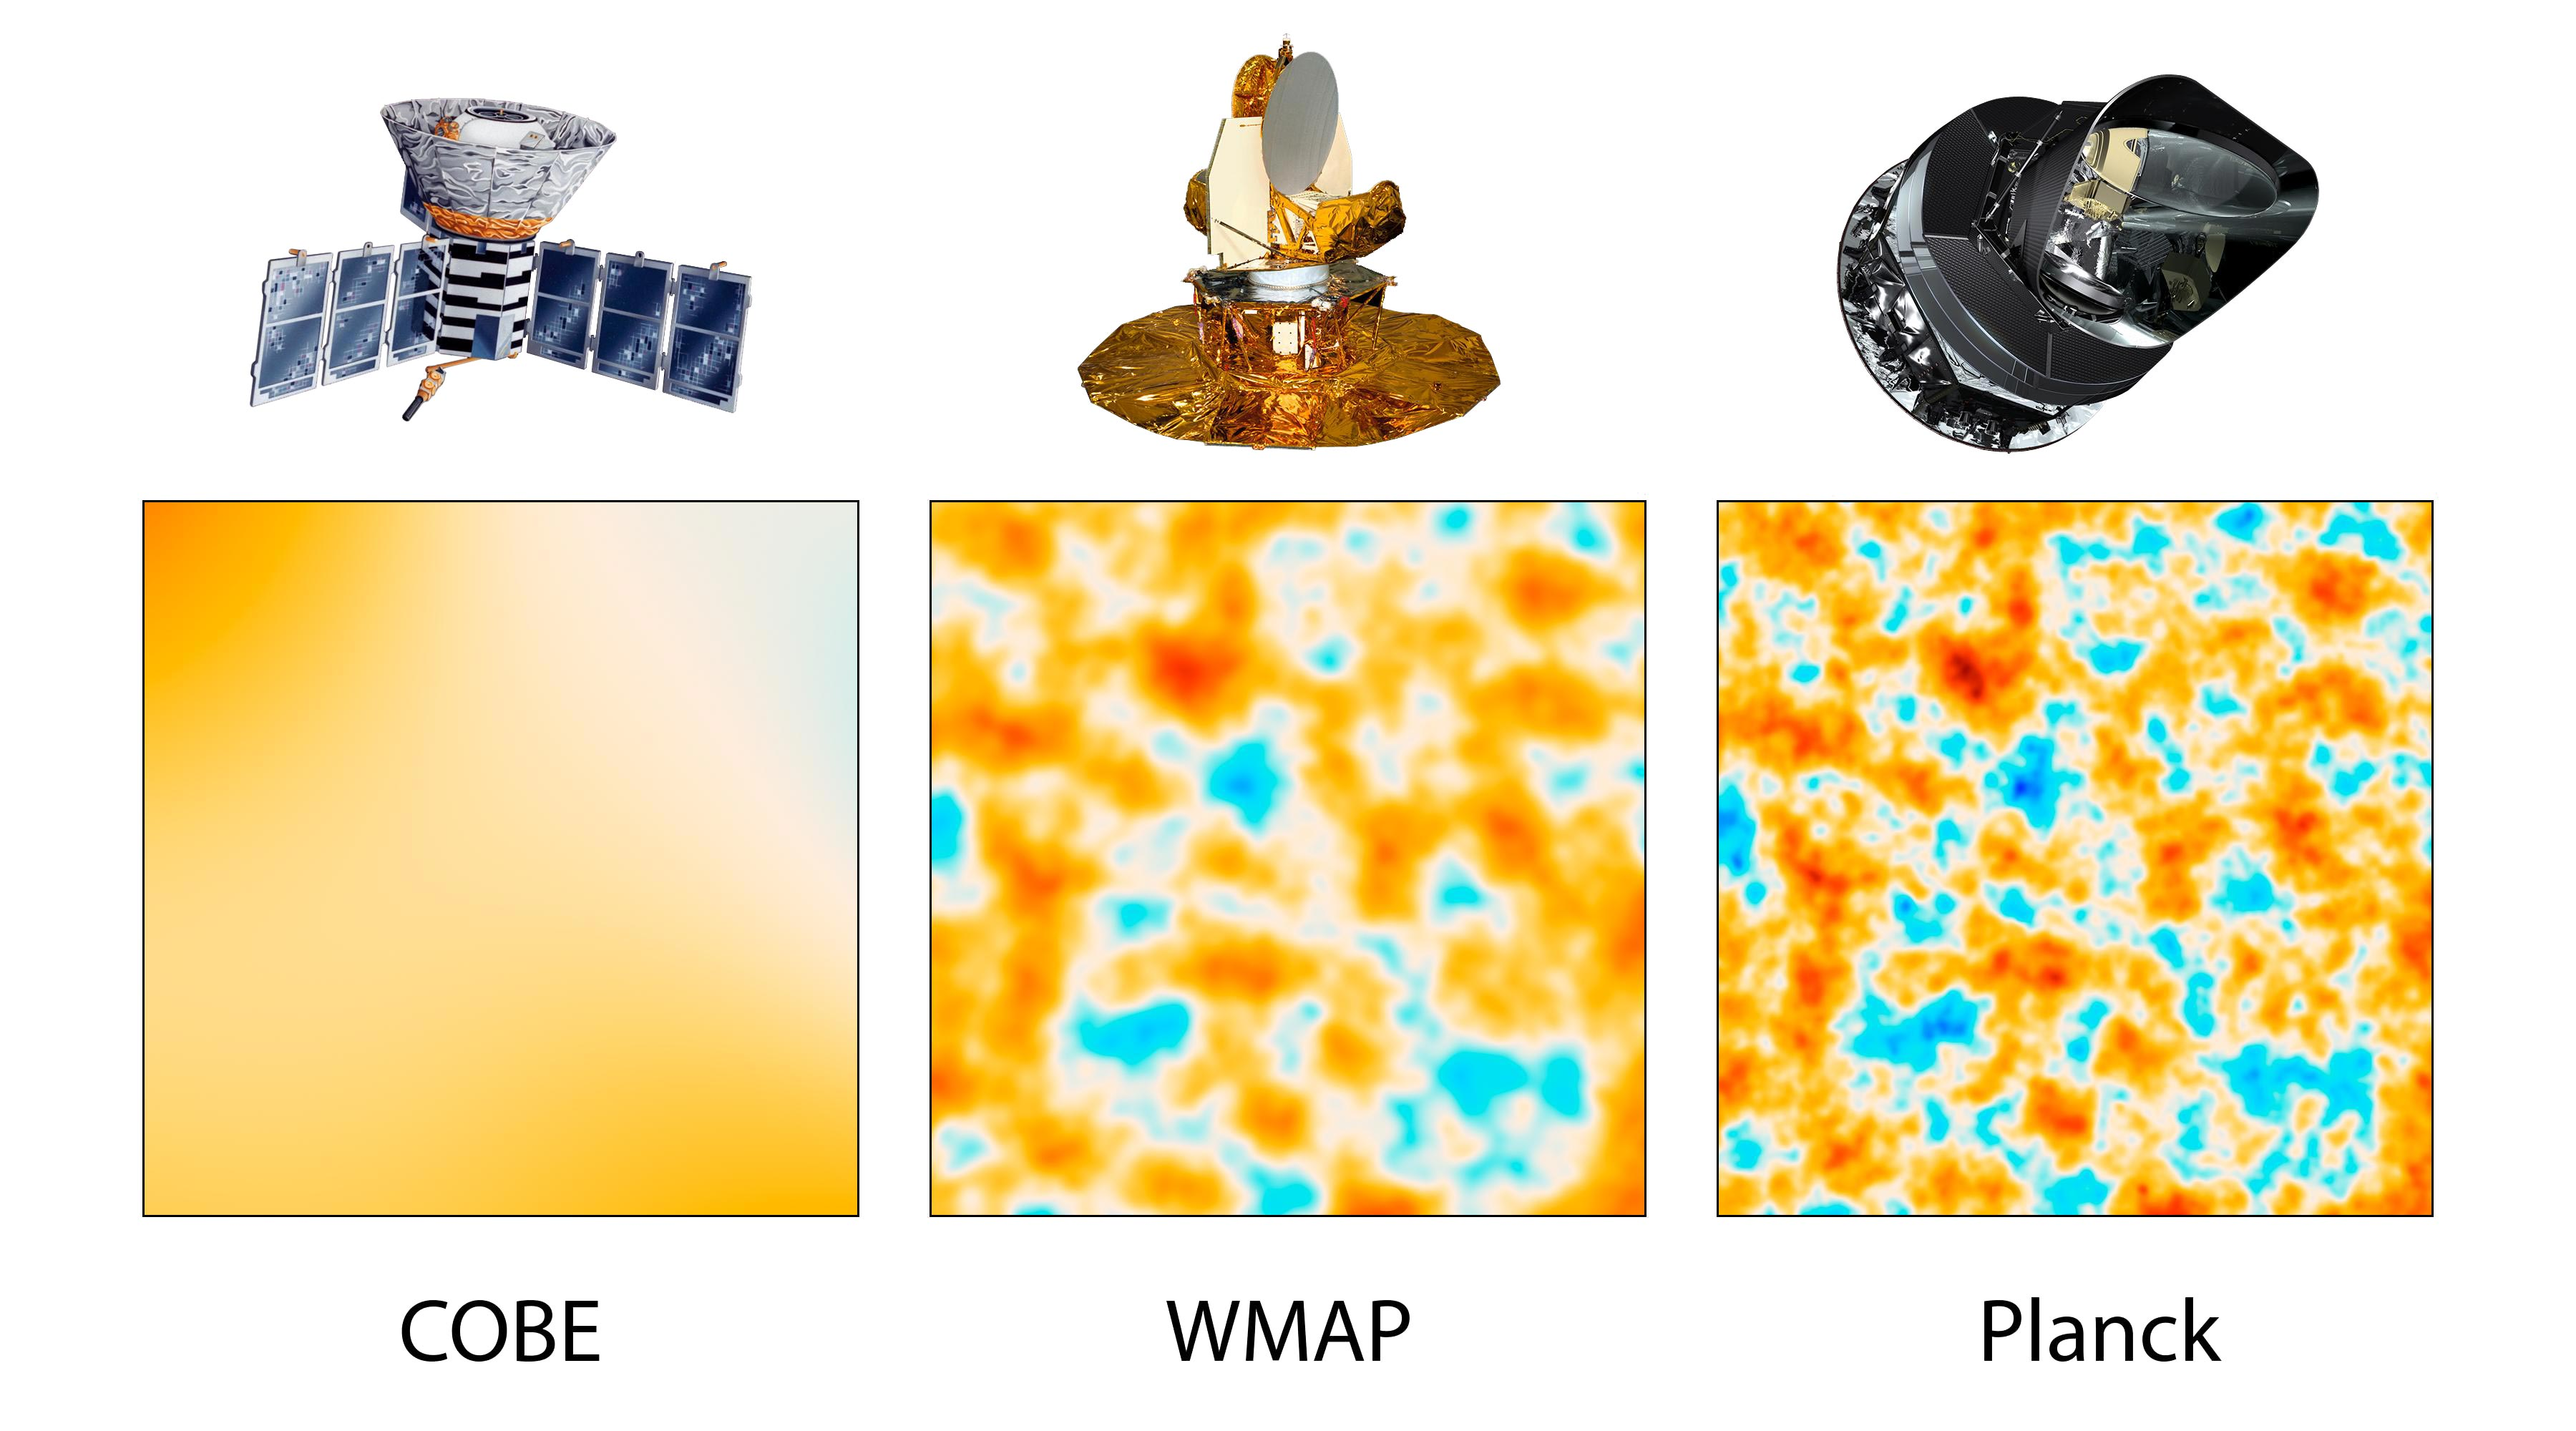
\includegraphics[width=0.9\textwidth]{CobeWmapPlanckComparison.jpg}
	
	\vspace{0.5in}
		
	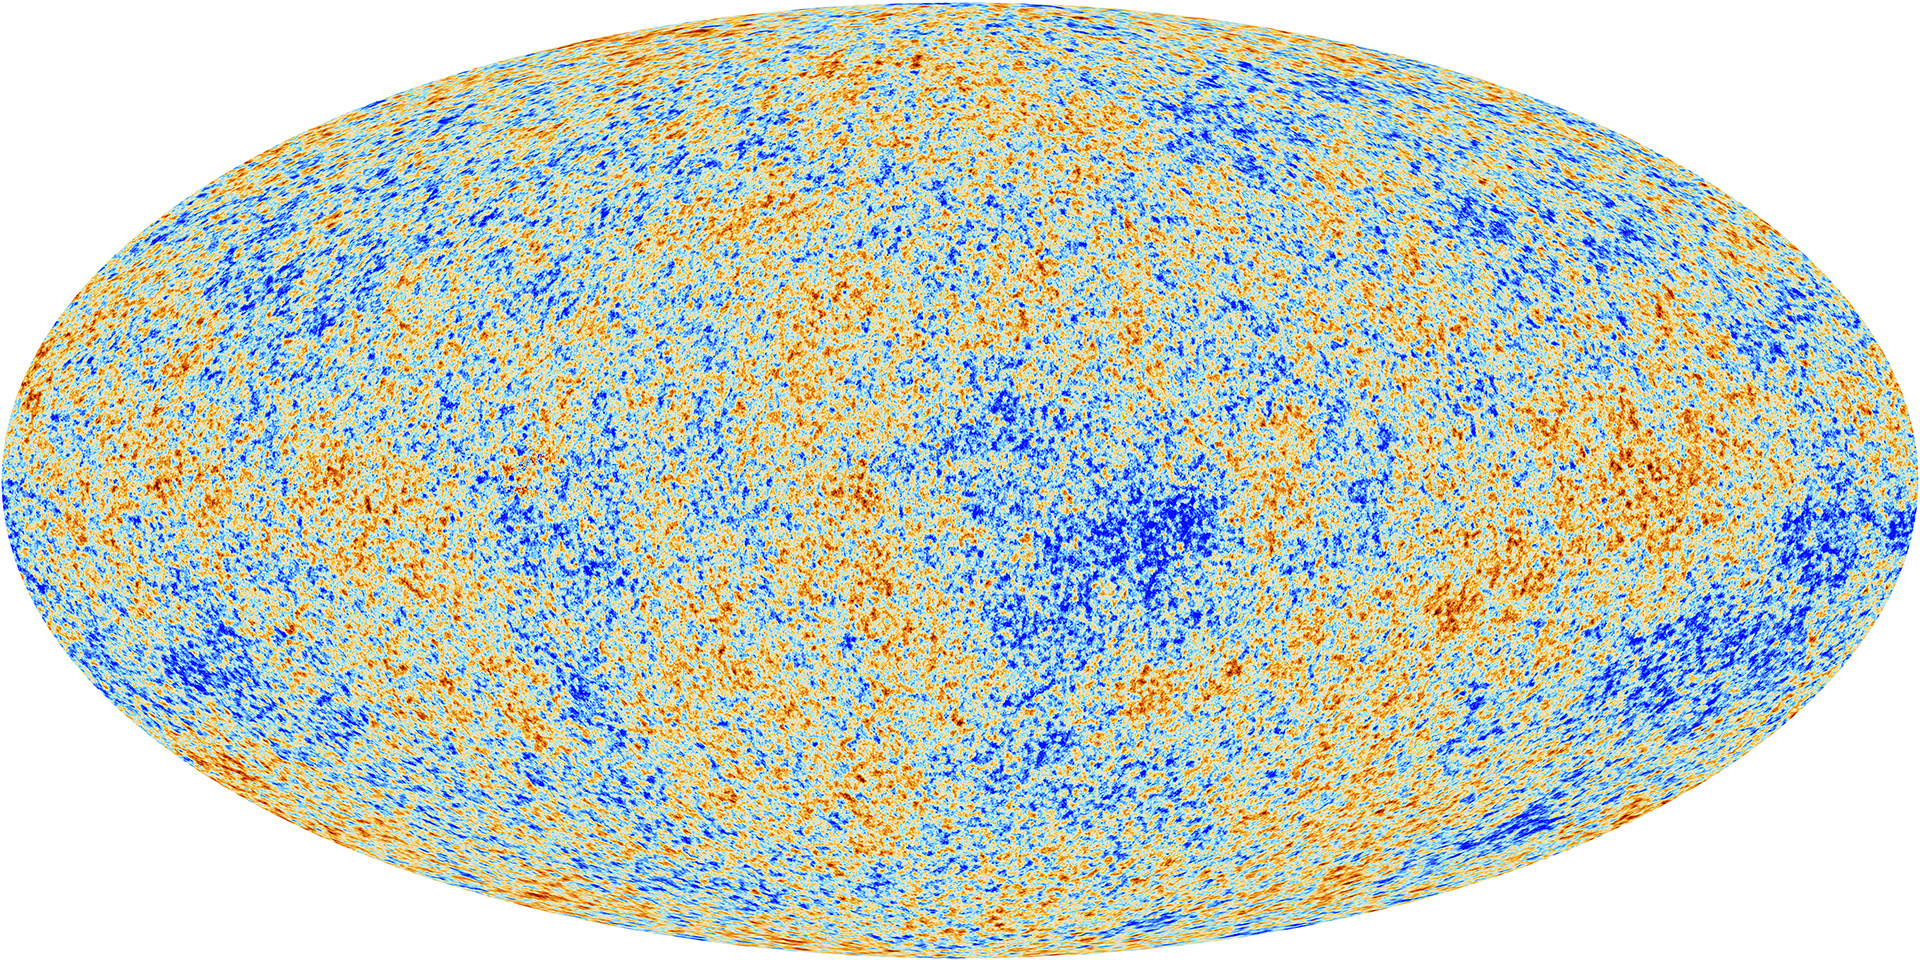
\includegraphics[width=0.8\textwidth]{Planck_CMB.jpg}
	
	{\sffamily Planck CMB}
	
	\caption[Short caption]{Top: Long caption Credit -- NASA/JPL-Caltech/ESA Bottom: Credit -- ESA and the Planck Collaboration}
\end{figure}

Imprinted by primordial quantum fluctuations,


Our current understanding of the Universe is of one consisting of $30.89 \pm 0.62\%$ matter and $69.11 \pm 0.62\%$
\citep{Collaboration:2015tp}

\section[Studying distant galaxies]{Studying distant galaxies}
\label{sec:section1_label}

QSOs at cosmological distances: \citet{Schmidt:1965gm}

Star-forming galaxies: \citep{Partridge:1967iw}

QSOs are $z \simgreat 4$
\citep{1990ApJ...357L...9G}

\citep{1992AJ....104..941S}

Normal star-forming galaxies at $z \simgreat 4$
\citep{Steidel:1995kx}
\citep{Steidel:1996jd}
\citep{1996MNRAS.283.1388M}

\citep{1999ApJ...519....1S}

\citep{Thompson:2001da}, \citep{Thompson:2003dp}, \citep{Fontana:2003ch}, \citep{Giavalisco:2004et}, \citep{Dickinson:2004ba}, \citep{Capak:2004im}, \citep{Stanway:2003fx}, \citep{Stanway:2004kr}

Text of chapter.  


\section{Estimating galaxy stellar masses}
Using the panchromatic spectral energy distribution (SED) of a galaxy to estimate its stellar mass (or other physical property of interest) has become an increasingly popular and powerful technique. At its simplest, the shape of a galaxy's SED tells us about the mass-to-light ratio, $\Mstar/L$, and therefore its overall normalisation can be used to estimate the corresponding total stellar mass. The shape of the SED itself (and hence the $\Mstar/L$) itself is a product of almost every underlying physical property of the galaxy which can tell as about both the past and present stellar population.

Firstly, the age of the underlying stellar population (and by association the galaxy's star-formation history) as well its metallicity and chemical enrichment history are encoded into the stellar emission. Secondly, the initial stellar emission is then processed by the surrounding gas and dust, so the observed SED is also a function of the distribution, mass and grain sizes of the dust within a galaxy.

Just what can be learned from the integrated light of a galaxy is highly dependent both on the quality of the data (including whether it is photometric or spectroscopic) and the model ingredients used to interpret that data.

...

When using SPS to interpret galaxy SEDs, the basic building blocks are simple stellar populations (SSPs) -- the SED of a single stellar population formed at the same time with a single metallicity and initial mass function (IMF). The construction of SSPs requires stellar spectral libraries and stellar isochrones for a given metallicity


Crucially, since the outputs of these models is simply the flux as a function of wavelength for a given set of population parameters, they can both be easily compared with each other and used in identical ways. With a suite of SSPs, composite stellar populations (CSPs) can then be constructed to simulate more complicated star-formation and metallicity histories along with the effects of 

In theory, $\text{SFR}(t)$ and $\text{P}(Z,t)$ can be arbitrarily complex. However, in practice this would require huge computational expense and with most data lead to minimal increase in accuracy for estimates of stellar masses over simpler model assumptions. Two such simplifications are commonly made, firstly that for a given composite stellar population the metallicity is fixed a single value. Secondly, the SFH can be parametrised as a simpler time dependent function with one or more parameters.

Most commonly used is a SFH which decays exponentially over some characteristic timescale, $\tau$, such that $\text{SFR}(t) \propto \exp(-t/\tau)$. More recently, it has been shown that rising star-formation models (e.g. negative $\tau$'s) are both a better a fit to the observed photometry of high-redshift galaxies \citep{Maraston:2010dl} and a better representation of the theoretical predictions from simulations \citep{2011MNRAS.410.1703F,Dayal:2013jm}.

OTHER SIMPLE PARAMETRISATIONS USED

Another novel approach to constructing plausible and accurate star-formation and metallicity history is that of Pacifici, whereby a large number of SFR and Z histories from semi-analytic models are used to construct a set of CSPs for fitting.

However the SFR and metallicity histories of models are parametrised, what is most important is that the chosen models can accurately represent the full dynamic range of observed galaxy photometry and give un-biased estimates of the stellar population properties we are interested in measuring. At $z > 3$, when the Universe is less than $\sim 2$ Gyr old, the limited ages of stars possible means that degeneracies introduced into SED fitting from the SFH alone are somewhat reduced. \citep{2013A&A...549A...4S} found...

METALLICITY

Another critical assumption in the use of SPS modelling is the choice of initial mass function. Without direct measurements of the IMF in distant galaxies, we are limited to the assumption of locally measured IMF such as the canonical \citet{Salpeter:1955hz} or \citet{Chabrier:2003ki} and \citet{Kroupa:2001ki} functions. 

\section{The CANDELS survey}
Regions of the sky which have been well studied by the \emph{Hubble} Space Telescope, such as the GOODS fields \citep{2004ApJ...600L..93G}, have become increasingly valuable resources for studying the evolution of galaxies and build-up of black holes through cosmic time. This is thanks to the ever-growing wealth of observations across the whole electromagnetic spectrum and the extreme depths reached by these observations.
However, the deep fields such as GOODS North and South cover only very small areas of the sky ($\sim 320$ arcmin$^{2}$ combined for Hubble data). This leads to large uncertainties in galaxy counts due to cosmic variance and also makes them poor for studying rare bright (/massive) objects.

While the deep optical coverage is allowed the Lyman break selection of galaxies out to $z\sim6$ and provided rest-frame optical morphologies of lower redshift galaxies, in order to extend this analysis to greater redshifts requires near-infrared observations of comparable depth to those existing at shorter wavelengths. Infrared surveys reaching to depths of $H_{160} \simgreat 26$ were possible with the NICMOS camera but were severely limited by the survey efficiency of the instrument with respect to its optical counter-part, ACS. The GOODS NICMOS Survey (GNS, ) observed parts of the GOODS North and South fields to a depth of $H_{160} \sim 26.5$ (cf. $V_{606} = 27.8$  \citep{2004ApJ...600L..93G}). Surveying XX arcmin$^{2}$ to this depth in just one single filter required 180 orbits of Hubble observations. Clearly, extending such a survey to more filters and significantly greater areas was not feasible with the existing facilities. Furthermore, using ground-based facilities the required depths are just not possible even with the largest 8m+ telescopes. 

Thankfully, the greatly improved capabilities of the Wide Field Camera 3 (WFC3), installed in \emph{Hubble} as part of the final service mission, such a task was made considerably more feasible. 

Efficiency plot

The CANDELS project (Cosmic Assembly Near-infrared Deep Extra-galactic Legacy Survey) leverages the new infrared capabilities to make observations which are both deeper and more extensive than previously available for the key legacy fields. ... awarded 900 orbits etc.

In the context of the many outstanding questions in galaxy formation and evolution, the CANDELS survey set out with a wide range of primary scientific goals in four key areas:

\begin{enumerate}
		\item \emph{Cosmic Dawn}: the formation and early evolution of galaxies ($z > 4$)
		\item \emph{Cosmic High Noon}: the peak of star-formation and AGN activity ($1 < z < 3$)
		\item Ultraviolet Observations: Host stars at $1 < z < 3.5$
		\item Supernovae: Standardizable candels beyond $z\sim1$
\end{enumerate}

\begin{quotation}
	``CD1	\quad Improve constraints on the bright end of the galaxy LF at $z \approx 7$ and 8 and make $z \approx 6$ measurements more robust.
Combine with WFC3/IR data on fainter magnitudes to constrain the UV luminosity density of the universe at the end of the reionization era
	
	CD2 \quad Constrain star formation rates, ages, metallicities, stellar masses, and dust contents of galaxies at the end of the
reionization era, $z \approx 6$ --10. Tighten estimates of the evolution of stellar mass, dust, and metallicity at $z = 4$-- 8 by combining WFC3 data with very deep Spitzer IRAC photometry"
\end{quotation}

The final survey program involved observations of five key extra-galactic survey fields -- GOODS South, GOODS North, the extended Groth strip (EGS), the UKIDSS Ultra Deep Survey (UDS) and the COSMOS field -- with observations of these fields split into two distinct tiers. The first (and deepest) of these tiers, hereafter CANDELS/Deep, is primarily comprised of observations over parts of the GOODS North and South (totalling XX) to a depth of $\sim 13$ Hubble orbits. The second shallower tier (CANDELS/Wide) consists of observations over all five fields to a depth of $\sim 2-3$ orbits per tile and covering YY.

The first deep field completed was the GOODS South field and was chosen as the basis for the majority of the analysis undertaken throughout this thesis. Full details of this dataset can be found in \citet{Guo:2013ig}, including the data reduction and homogenisation of the respective space and ground-based ancillary data. 

\section{Thesis Outline}
%% %% End of file...  %%
